\documentclass[a4paper]{article}

\usepackage[english]{babel}
\usepackage[utf8]{inputenc}
\usepackage{amsmath}
\usepackage{graphicx}
\usepackage[colorinlistoftodos]{todonotes}

\title{Behaviour Dynamics in Social Networks - Assignment 1}

\author{Maria Hotoiu, Federico Tavella}

\date{\today}

\begin{document}
\maketitle

\begin{abstract}
After Jenny has entered Mark’s door, her presence clearly makes that Mark becomes happy. Liking Mark a lot, his happiness makes her nervous, which makes that she breaks one of the two nice vases near the door. Seeing this, Mark becomes angry on her. This makes Jenny sad. Jenny’s sadness makes Mark’s anger disappear, and he gives Jenny a hug. Seeing this, Mark’s partner Dion becomes jealous, upon which she breaks the other vase.
\newline
Use the concepts and formats introduced in Chapter 2 to analyse and model this scenario by a temporal-causal network by the following steps.
\end{abstract}

\section{Graphical conceptual representation}
\label{sec:graphical_conceptual_representation}

States describing the scenario:

\begin{enumerate}
\item Jenny's presence ($X_1$);
\item Mark becomes happy ($X_2$);
\item Jenny likes Mark ($X_3$);
\item Jenny becomes nervous ($X_4$);
\item Jenny breaks a vase ($X_5$);
\item Mark becomes angry ($X_6$);
\item Jenny becomes sad ($X_7$);
\item Mark gives Jenny a hug ($X_8$);
\item Dion become jealous ($X_9$);
\item Dion breaks a vase ($X_10$).
\end{enumerate}

In Figure~\ref{fig:graphical_conceptual_representation}, we can observe a connection that models a negative impact in order to make the level of the affected state lower - the one going from $X_7$ to $X_6$ (i.e. Mark anger decreases due to Jenny sadness). There is also a loop that contains two states: $X_6$ and $X_7$.


\begin{figure}[!htbp]
\center
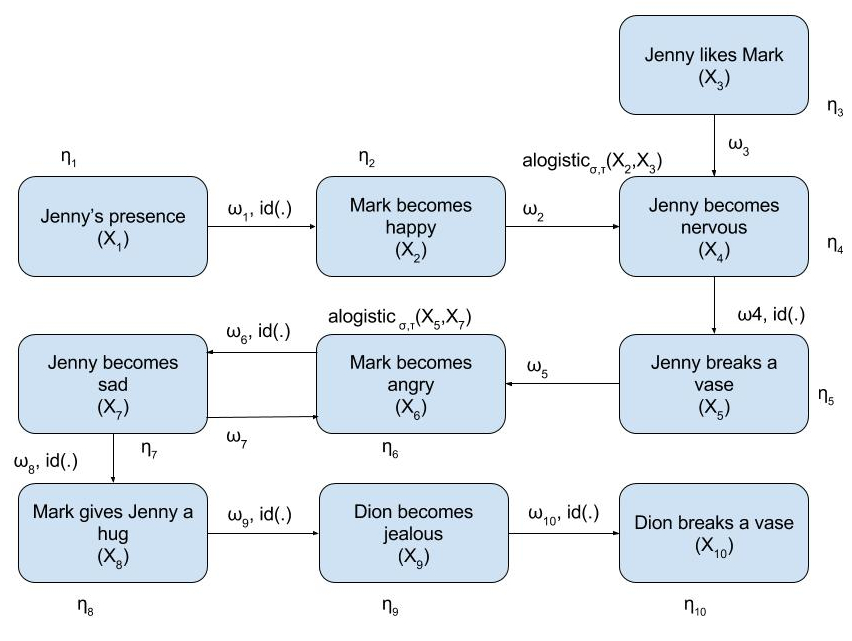
\includegraphics[width=0.95\textwidth]{res/img/graphical_conceptual_representation}
\caption{Conceptual representation of the scenario.}
\label{fig:graphical_conceptual_representation}
\end{figure}

\section{Conceptual representation in matrix format}

We now move to the matrix representation of the graph in Figure~\ref{fig:graphical_conceptual_representation}. Rows represent nodes from which edges are starting, while columns represent nodes in which edges are ending.

\begin{figure}[!htbp]
\centering
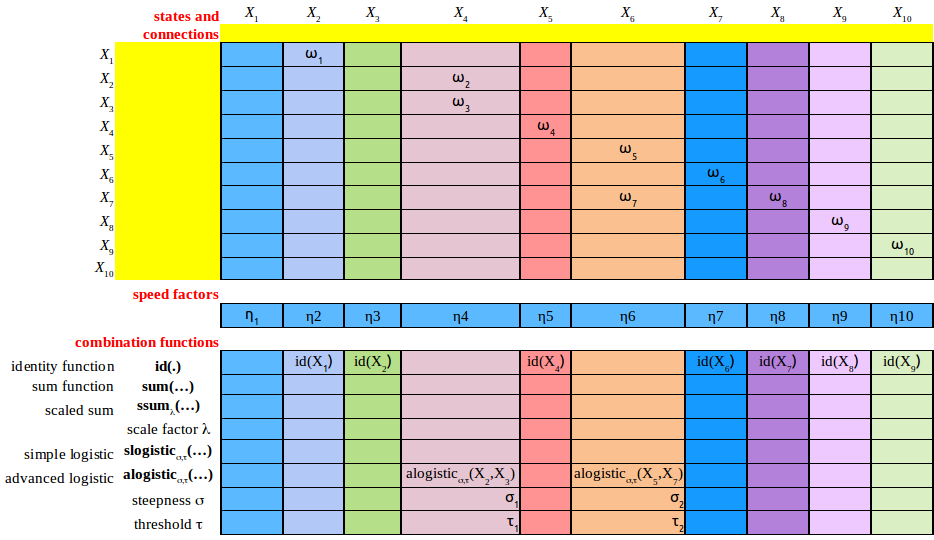
\includegraphics[width=0.95\textwidth]{res/img/matrix_conceptual_representation}
\caption{Matrix format of the conceptual representation}
\label{fig:matrix_conceptual_representation}
\end{figure}

\section{Numerical representation}

Numerical representation for the scenario represented in Figure \ref{fig:matrix_conceptual_representation}.

\subsection{Difference equation}

Initial states:
\begin{equation}
X_{1}(t+\Delta t) = X_{1}(t) + \eta_{1} ( id(X_{1}(t)) - X_{1}(t))\Delta t = X_{1}(t)
\end{equation}
\begin{equation}
X_{3}(t+\Delta t) = X_{3}(t) + \eta_{3} ( id(X_{3}(t)) - X_{3}(t))\Delta t = X_{3}(t)
\end{equation}
\\
Intermediate states:
\begin{equation}
X_{2}(t+\Delta t) = X_{2}(t) + \eta_{2} (id(\omega_{2} X_{1}(t)) - X_{2}(t))\Delta t
\end{equation}
\begin{equation}
X_{4}(t+\Delta t) = X_{4}(t) + \eta_{4} ( alogistic_{\sigma ,\tau}(\omega_{2} X_{2}(t),\omega_{3} X_{3}(t)) - X_{4}(t))\Delta t
\end{equation}
\begin{equation}
X_{5}(t+\Delta t) = X_{5}(t) + \eta_{5} (id(\omega_{4} X_{4}(t)) - X_{5}(t))\Delta t
\end{equation}
\begin{equation}
X_{6}(t+\Delta t) = X_{6}(t) + \eta_{6} (alogistic_{\sigma ,\tau}(\omega_{5} X_{5}(t),\omega_{7} X_{7}(t)) - X_{6}(t))\Delta t
\end{equation}
\begin{equation}
X_{7}(t+\Delta t) = X_{7}(t) + \eta_{7} (id(\omega_{6} X_{6}(t)) - X_{7}(t))\Delta t
\end{equation}
\begin{equation}
X_{8}(t+\Delta t) = X_{8}(t) + \eta_{8} (id(\omega_{8} X_{7}(t)) - X_{8}(t))\Delta t
\end{equation}
\begin{equation}
X_{9}(t+\Delta t) = X_{9}(t) + \eta_{9} (id(\omega_{9} X_{8}(t)) - X_{9}(t))\Delta t
\end{equation}
\\
Final state:
\begin{equation}
X_{10}(t+\Delta t) = X_{10}(t) + \eta_{10} (id(\omega_{10} X_{9}(t)) - X_{10}(t))\Delta t
\end{equation}


\subsection{Differential equation}

Initial states:
\begin{equation}
\frac{\delta X_{1}(t)}{\delta t} = X_{1}(t) + \eta_{1} \cdot ( id(X_{1}(t)) - X_{1}(t))
\end{equation}
\begin{equation}
\frac{\delta X_{3}(t)}{\delta t} = X_{3}(t) + \eta_{3} \cdot ( id(X_{3}(t)) - X_{3}(t))
\end{equation}
\\
Intermediate states:
\begin{equation}
\frac{\delta X_{2}(t)}{\delta t} = X_{2}(t) + \eta_{2} \cdot ( id(X_{1}(t)) - X_{2}(t))
\end{equation}
\begin{equation}
\frac{\delta X_{4}(t)}{\delta t} = X_{4}(t) + \eta_{4} \cdot ( alogistic_{\sigma ,\tau}(\omega_{2} X_{2}(t),\omega_{3} X_{3}(t)) - X_{4}(t))
\end{equation}
\begin{equation}
\frac{\delta X_{5}(t)}{\delta t} = X_{5}(t) + \eta_{5} \cdot ( id(X_{4}(t)) - X_{5}(t))
\end{equation}
\begin{equation}
\frac{\delta X_{6}(t)}{\delta t} = X_{6}(t) + \eta_{6} \cdot (alogistic_{\sigma ,\tau}(\omega_{5} X_{5}(t),\omega_{7} X_{7}(t)) - X_{6}(t))
\end{equation}
\begin{equation}
\frac{\delta X_{7}(t)}{\delta t} = X_{7}(t) + \eta_{7} \cdot ( id(X_{6}(t)) - X_{7}(t))
\end{equation}
\begin{equation}
\frac{\delta X_{8}(t)}{\delta t} = X_{8}(t) + \eta_{8} \cdot ( id(X_{7}(t)) - X_{8}(t))
\end{equation}
\begin{equation}
\frac{\delta X_{9}(t)}{\delta t} = X_{9}(t) + \eta_{9} \cdot ( id(X_{8}(t)) - X_{9}(t))
\end{equation}
\\
Final state:
\begin{equation}
\frac{\delta X_{10}(t)}{\delta t} = X_{10}(t) + \eta_{10} \cdot ( id(X_{9}(t)) - X_{10}(t))
\end{equation}

\section{Expected behaviour}\label{sec:expected_behaviour}

There are two constant and non-zero states at $t = 0$: Jenny's presence ($X_{1}$) and Jenny liking of Mark ($X_{3}$). All the others states ($X_{2}$, $X_{4}$, $X_{5}$, $\ldots$, $X_{10}$) are starting at $0$. We expect the behaviour of the network as follows: it starts with Jenny's presence as non-zero, which makes Mark's happiness go from low to high. This change, together with the constant factor of Jenny liking Mark, make Jenny's nervousness go from low to high, which makes her break a vase (Jenny's vase breaking goes from low to high). As a consequence of the breaking, Mark's anger goes from low to high, which makes Jenny's sadness also go from low to high. This change in Jenny's sadness makes Mark's anger go from high back to low and it also makes Mark's hugging of Jenny go from low to high. The change in the hugging state makes Dion's jealousy go from low to high and as a consequence she breaks a vase (Dion's vase breaking goes from low to high). During all these processes, we can observe temporal-causal relationships between nodes connected by edges.

\begin{figure}[!ht]
\center
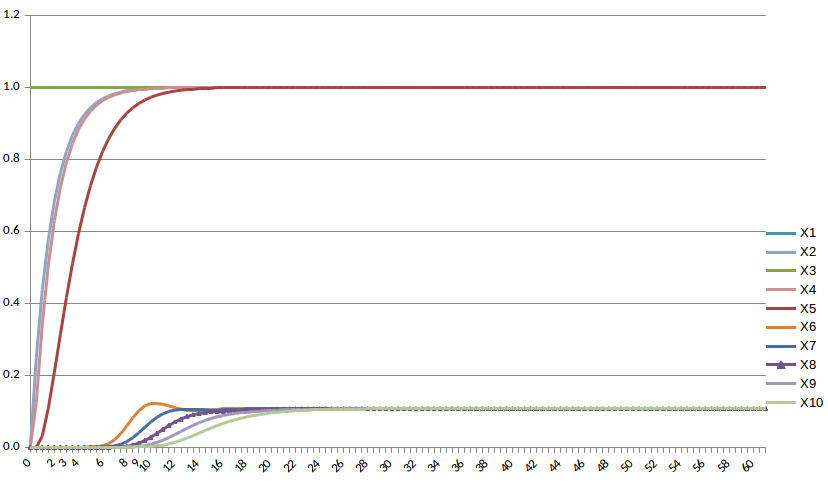
\includegraphics[width=\textwidth]{res/img/numerical_representation}
\caption{Results obtained from the simulation of the scenario. All the edges are weighted the same ($\omega_{i} = 1$), except for $\omega_{7} = -1$. They also share the same speed factor: $\eta_{i} = 0.5,  i = 1 \ldots 10$. The \textit{alogistic} function is set with $\sigma = 10$ and $\tau = 1$}
\label{fig:numerical_representation}
\end{figure}

\section{Simulation}

In this section, we analyze the experimental results too check if they are coherents with the expected behaviour described in Section \ref{sec:expected_behaviour}. As we can see in Figure~\ref{fig:numerical_representation}, the two costant states - $X_{1}$ and $X_{3}$ - are set to 1. The states connected to them ($X_{2}$ and $X_{4}$) are activated due to a \textit{causal relationship}. Moreover, we can see how the connection that models the negative impact (i.e. the edge from $X_{7}$ to $X_{6}$) lowers the value of $X_{6}$ around $t = 10$. Finally, we observe how the loop lead to a convergence of values of all the involved nodes - $X_{6}$ and $X_{7}$, and consequently $X_{8}$, $X_{9}$ and $X_{10}$.





\begin{thebibliography}{9}
\bibitem{nano3}
  Treur, J.,
  \emph{Network-Oriented Modeling: Addressing Complexity of Cognitive, Affective and Social Interactions}.
  Series on Understanding Complex Systems, Springer Publishers, October 2016.

\end{thebibliography}
\end{document}
